% start the document

% specify the document layout and font size
\documentclass[preprint,12pt]{elsarticle}
% \documentclass[final,twocolumn,12pt]{elsarticle}
% \usepackage[margin=1.5cm,includefoot]{geometry}
\usepackage{setspace}

% uploading packages
\usepackage{graphicx}
\usepackage{amssymb}
\usepackage{textcomp} % https://latex.org/forum/viewtopic.php?f=4&t=3364#p13124, https://tex.stackexchange.com/questions/165115
\usepackage{gensymb}
\usepackage{lineno}
\usepackage{mathtools}
\usepackage[title]{appendix}
\usepackage{pgfmath}
\newcommand{\calcnum}[1]{%
    \pgfmathparse{#1}%
    \num[round-mode=places,round-precision=1]{\pgfmathresult}%
}
\usepackage[separate-uncertainty=true]{siunitx} % \usepackage{xr-hyper} %needs to  be before hyperref
\usepackage{xurl} %needs to be before hyperref
\usepackage[colorlinks]{hyperref}
\hypersetup{breaklinks=true} % set automatically by hyperref?
% \PassOptionsToPackage{hyphens}{url}\usepackage{hyperref} %allow URLs to break across lines
\usepackage[nameinlink,capitalise]{cleveref} %needs to appear after hyperref, https://tex.stackexchange.com/questions/396728/my-equations-referencing-not-working
\Crefname{figure}{Figure}{Figures} %needs to appear after hyperref and cleveref
\crefname{appsec}{Appendix}{Appendices}
\newcommand\crefrangeconjunction{--} % modify the reference style
\usepackage{mathrsfs}
\usepackage{enumitem}
\usepackage{tabulary}
\usepackage{caption}
\usepackage{subcaption}
\usepackage{multirow}
\usepackage{makecell} % https://tex.stackexchange.com/questions/2441/how-to-add-a-forced-line-break-inside-a-table-cell
\newcommand{\NA}{---} % holds an m-dash
\graphicspath{{figures/}} %Setting the graphicspath
% ---------to deal with the double quotes----------- 
\usepackage [english]{babel}
\usepackage [autostyle, english = american]{csquotes}
\MakeOuterQuote{"}
\usepackage{listings}[breakatwhitespace=true,escapechar=\%]
\usepackage{matlab-prettifier}
\newcommand{\matlab}[1]{\mbox{\lstinline[style=Matlab-editor]{#1}}}
%alternatively can use `` '' format for double quotes
\usepackage{booktabs}
\setlength{\abovetopsep}{1ex}
\usepackage[shortcuts,abbreviations]{glossaries-extra}
\newcommand*{\TCac}[1]{\ecapitalisewords{\glsentrylong{#1}}}
% remove the "Preprint submitted to Elsevier" footer on the first page
\makeatletter
\def\ps@pprintTitle{%
   \let\@oddhead\@empty
   \let\@evenhead\@empty
   \def\@oddfoot{\reset@font\hfil\thepage\hfil}
   \let\@evenfoot\@oddfoot
}
\makeatother

% Cross referencing with the xr package in Overleaf (https://www.overleaf.com/learn/how-to/Cross_referencing_with_the_xr_package_in_Overleaf)
\makeatletter
\newcommand*{\addFileDependency}[1]{% argument=file name and extension
  \typeout{(#1)}
  \@addtofilelist{#1}
  \IfFileExists{#1}{}{\typeout{No file #1.}}
}
\makeatother
\newcommand*{\myexternaldocument}[1]{%
    \externaldocument{#1}%
    \addFileDependency{#1.tex}%
    \addFileDependency{#1.aux}%
}

\usepackage{nameref,zref-xr}
\zxrsetup{toltxlabel}
%https://tex.stackexchange.com/questions/77774/undefined-control-sequence-when-cross-referencing-with-xr-hyper
% \myexternaldocument{supp}

\biboptions{sort&compress}
\interfootnotelinepenalty=10000 %prevent footnotes from getting split across columns/pages 
%\patchcmd{\emailauthor}{(#2)}{(S.G. Baird).}{}{} %Removes/Abbreviates corresponding author name after Email address so that the footnote doesn't take up 2 lines.
% Double Spacing
% \doublespacing
\usepackage[margin=1.5cm,includefoot]{geometry}
\usepackage{auto-paper}
% \PassOptionsToPackage{refcheck}{auto-paper} %comment this out before submission

\zexternaldocument*{main-frankenstein-2} %try deleting log files if producing an error, see https://tex.stackexchange.com/questions/131709/unclean-aux-file-causes-file-ended-while-scanning-use-of-newlbel-error-wh
% Concatenate the different "values" .tex files
%RMSE values
% \newcommand{\baryrmse}{0.0242}
% \newcommand{\gprrmse}{0.0220}
% \newcommand{\idwrmse}{0.0345}
% \newcommand{\nnrmse}{0.0448}
% \newcommand{\avgrmse}{0.1302}
% %paper-data6
% \newcommand{\baryrmse}{0.0238}
% \newcommand{\gprrmse}{0.0218}
% \newcommand{\idwrmse}{0.0356}
% \newcommand{\nnrmse}{0.0445}
% \newcommand{\avgrmse}{0.1283}
%\newcommand{\gprrmsePercReduction}{83}
% paper-data9
\newcommand{\baryrmse}{0.0239}
\newcommand{\gprrmse}{0.0217}
\newcommand{\idwrmse}{0.0343}
\newcommand{\nnrmse}{0.0448}
\newcommand{\avgrmse}{0.1284}
\newcommand{\gprrmsePercReduction}{83.1}

%MAE values
% \newcommand{\barymae}{0.0145}
% \newcommand{\gprmae}{0.0145}
% \newcommand{\idwmae}{0.0223}
% \newcommand{\nnmae}{0.0307}
% \newcommand{\avgmae}{0.0965}
% %paper-data6
% \newcommand{\barymae}{0.0145}
% \newcommand{\gprmae}{0.0145}
% \newcommand{\idwmae}{0.0225}
% \newcommand{\nnmae}{0.0307}
% \newcommand{\avgmae}{0.0955}
%paper-data9
\newcommand{\barymae}{0.0145}
\newcommand{\gprmae}{0.0145}
\newcommand{\idwmae}{0.0223}
\newcommand{\nnmae}{0.0308}
\newcommand{\avgmae}{0.0959}

%\newcommand{\nnomega}{2.8709 \pm 0.69112}
\newcommand{\nnomega}{2.8702 \pm 0.69117}

\newcommand{\symtime}{76}

\newcommand{\nigprbrkrmse}{0.1471}

%Supplementary
\newcommand{\thr}{\SI{1.1}{\joule\per\square\meter}}
\newcommand{\sigthr}{\SI{1.1}{\joule\per\square\meter}}
\newcommand{\thrtwo}{\SI{1.2}{\joule\per\square\meter}}


%% main-frankenstein-2
\newcommand{\minsymdist}{$\sim$\SI{64.0}{\tobydeg}}
\newcommand{\percExplained}{$\sim$\SI{99.6}{\percent}}
\newcommand{\percFiveVsOne}{$\sim$\SI{70}{\percent}}
\newcommand{\dimOne}{$\sim$\SI{65}{\tobydeg}}

% figure info, etc. that can dynamically change (color of points, etc.)
\newcommand{\startpt}{red points}
\newcommand{\singlept}{magenta points}
\newcommand{\sympt}{dark blue points}
\newcommand{\singlesympt}{dark blue point}
\newcommand{\refpt}{white circle}
\newcommand{\vbordercolor}{black}
\newcommand{\vcellcolor}{light blue}
\newcommand{\inpt}{input}
\newcommand{\outpt}{prediction}
% \newcommand{\inptvar}{ninputpts}
% \newcommand{\distfn}{GBdist4}
\newcommand{\vfzorepo}{\gls{vfz} repository}
\newcommand{\mytitleone}{Five Degree-of-Freedom Property Interpolation of Arbitrary Grain Boundaries via \glsentrytitlecase{vfz}{long} Framework}
% \newcommand{\mytitletwo}{Properties of a \glsentrytitlecase{5dof}{long} \glsentrytitlecase{fz}{long} defined via \glsentrytitlecase{vfz}{long} Framework}
\newcommand{\mytitletwo}{$O_h$ \glsentrytitlecase{5dof}{long} \glsentrytitlecase{fz}{long} Properties via \glsentrytitlecase{vfz}{long} Framework}
\makeglossaries
\GlsXtrEnableEntryCounting{abbreviation}{3}
% \glssetcategoryattribute{abbreviation}{indexonlyfirst}{true}
\glssetcategoryattribute{abbreviation}{nohyper}{true}

% \setabbreviationstyle[abbreviation]{long-short}

% \glsenableentrycount
% \glssetcategoryattribute{abbreviation}{entrycount}{2}

\newabbreviation[longplural=five degrees of freedom]{5dof}{5DOF}{five degree-of-freedom}
\newabbreviation[longplural=three degrees of freedom]{3dof}{3DOF}{three degree-of-freedom}
\newabbreviation[longplural=degrees of freedom]{dof}{DOF}{degree of freedom}
\newabbreviation{ebsd}{EBSD}{electron backscatter diffraction}
\newabbreviation[longplural={grain boundaries}]{gb}{GB}{grain boundary}
\newabbreviation{fcc}{FCC}{face-centered cubic}
\newabbreviation{sem}{SEM}{scanning electron microscope}
\newabbreviation{fea}{FEA}{finite element analysis}
\newabbreviation{bcs}{BCs}{boundary conditions}
\newabbreviation[longplural={triple junctions}]{tj}{TJ}{triple junction}
\newabbreviation{gpr}{GPR}{Gaussian process regression}
\newabbreviation{gprm}{GPRM}{Gaussian process regression mixture}
\newabbreviation{ann}{ANN}{artificial neural network}
\newabbreviation{nn}{NN}{nearest neighbor}
\newabbreviation{rmse}{RMSE}{root mean square error}
\newabbreviation{mae}{MAE}{mean absolute error}
\newabbreviation{brk}{BRK}{Bulatov Reed Kumar}
\newabbreviation{gbed}{GBED}{grain boundary energy distribution}
\newabbreviation{gbcd}{GBCD}{grain boundary character distribution}
\newabbreviation{mfz}{MFZ}{misorientation fundamental zone}
\newabbreviation{bp}{BP}{boundary plane}
\newabbreviation{bpfz}{BPFZ}{boundary plane fundamental zone}
\newabbreviation{knn}{kNN}{k-nearest neighbor}
\newabbreviation{gbe}{GBE}{grain boundary energy}
\newabbreviation{gbo}{GBO}{grain boundary octonion}
\newabbreviation{nbo}{NBO}{no-boundary octonion}
\newabbreviation{oslerp}{oSLERP}{octonion Spherical Linear Interpolation}
\newabbreviation{loocv}{LOOCV}{leave-one-out cross validation}
\newabbreviation{kfcv}{kFCV}{k-fold cross validation}
\newabbreviation{seo}{SEO}{symmetrically equivalent octonion}
\newabbreviation{fex}{FEX}{file exchange}
\newabbreviation{idw}{IDW}{inverse-distance weighting}
\newabbreviation{fic}{FIC}{fully independent conditional}
\newabbreviation{svd}{SVD}{singular value decomposition}
\newabbreviation{gbc}{GBC}{grain boundary character}
\newabbreviation{fz}{FZ}{fundamental zone}
% \newabbreviation{pfz}{pFZ}{pseudo fundamental zone} % pfz replaced by vfz
% \newabbreviation{cmo}{CMO}{closed-mesh octonion} % cmo replaced by vfzo
\newabbreviation{vfz}{VFZ}{Voronoi fundamental zone}
\newabbreviation{vfzgbo}{VFZ-GBO}{Voronoi fundamental zone grain boundary octonion}
\newabbreviation{lobpcg}{LOBPCG}{locally optimal block preconditioned conjugate gradient}
\newabbreviation{lkr}{LKR}{Laplacian kernel regression}
\newabbreviation{ms}{MS}{molecular statics}
\newabbreviation{sst}{SST}{standard stereographic triangle}
\newabbreviation{ml}{ML}{machine learning}
\newabbreviation{doe}{DoE}{design of experiments}
\newabbreviation{ct}{CT}{coherent-twin}
% example abbreviations
% \newabbreviation{seo}{SEO}{symmetrically equivalent octonions}
%\newabbreviation[longplural={grain boundaries}]{gb}{GB}{grain boundary}

%example usage: \gls{gpr}
%example usage: \Gls{gpr} (capitalize first letter, only meaningful for first usage)
% \glspl{seo} --> symmetrically equivalent octonions OR SEOs
%^^^^^^^^^^^^^^^^^^^^^^^^^^^^^^^^^^^^^^^^^^^^^^^^^^^


% Add "S" to figure captions, sections, and equations
\renewcommand{\thefigure}{S\arabic{figure}}
\renewcommand{\thesection}{S\arabic{section}}
\renewcommand{\theequation}{S\arabic{equation}}

\begin{document}
	\sloppy %maybe deals with figure/text spacing. Should deal with text going off the page
	
	\begin{frontmatter}
		
		%\title{Grain Boundary Octonion Meshing and Interpolation}
		\title{\mytitletwo{}: Supplementary Information}
		
		\author[myu]{Sterling G. Baird\corref{cor1}}
\ead{ster.g.baird@gmail.com}
\author[myu]{Eric R. Homer}
\author[myu]{David T. Fullwood}
\author[myu]{Oliver K. Johnson}

\address[myu]{Department of Mechanical Engineering, Brigham Young University, Provo, UT 84602, USA}

\cortext[cor1]{Corresponding author.}

\date{October 2021}
		
	\end{frontmatter}
	
\tableofcontents

\section{Brief Summary of \glsxtrshort{vfz} Methods}

    We summarize the following aspects of the \gls{vfz} framework:
    \begin{itemize}
        \item Creation and definition of a \gls{vfz}
        \item Mapping \glspl{gb} to the \gls{vfz}
        \item Distance calculations
        \item Interpolation
        \item Comparison with traditional \gls{gbo} metric
    \end{itemize}
    Each of these is described in greater detail in \citet{bairdFiveDegreeofFreedomPropertyUnderReview}.
    
    To define a \gls{vfz}, an arbitrary, fixed, low-symmetry reference \gls{gbo} is chosen ($o_{\text{ref}}$) and for our use of \glspl{gbo}, the \gls{vfz} is defined as the region of $\mathbb{S}^7$ (the unit 7-sphere in 8 dimensions) closer to $o_{\text{ref}}$ than any of its symmetric images. If a low-symmetry \gls{gb} is chosen, the point within a \gls{vfz} will be unique within numerical tolerance (and hence it is a true \gls{fz}). Additionally, we use a Euclidean approximation to the true geodesic distance.
    
    
    A \gls{gbo} is composed of two quaternions, with the \gls{bp} normal in the $+z$ direction \cite{francisGeodesicOctonionMetric2019}. A \gls{gbo} is mapped into a \gls{vfz} by calculating the pairwise distances between the reference \gls{gbo} and each of the \glspl{seo}\footnote{Contrary to \citet{francisGeodesicOctonionMetric2019} which uses the passive convention for misorientation, we employ the active convention \cite{bairdFiveDegreeofFreedomPropertyUnderReview}. } and taking the \gls{seo} closest to the reference \gls{gbo}.
    
    Once a \gls{gbo} has been mapped into a \gls{vfz}, distance calculations proceed without further consideration of \glspl{seo}. The \gls{vfz} framework suffers from occasional, large distance overestimation which imposes a local sparseness of data and lead to poorer interpolation near the borders of a \gls{vfz}. However, this can be mitigated through ensemble or data augmentation techniques.
    
    Note that in the original definition of the \gls{vfz}, the authors examined different interpolation techniques \cite{bairdFiveDegreeofFreedomPropertyUnderReview}. In the present work, we focus on \gls{gpr} which in our case imposes the assumption that crystallographically similar \glspl{gb} share similar \glspl{gbe} within some correlation length. \Gls{gpr} has the added benefit of built-in uncertainty quantification.
    
    The primary differences between the \gls{vfz} framework and traditional \gls{gbo} distance metric are that the \gls{vfz} framework is defined by a continuous set of points, exhibits occasional distance overestimation, uses a Euclidean approximation, and has a lower computational complexity.

% \section{Nearest Neighbor Distances within a Large Point Set}

%     \Cref{fig:nnhist-knn-50000}a and b show a histogram of \num{50000} first \gls{nn} distances and the average distance for the k-th \gls{nn}.
    
% 	\begin{figure*}
% 		\centering
% 		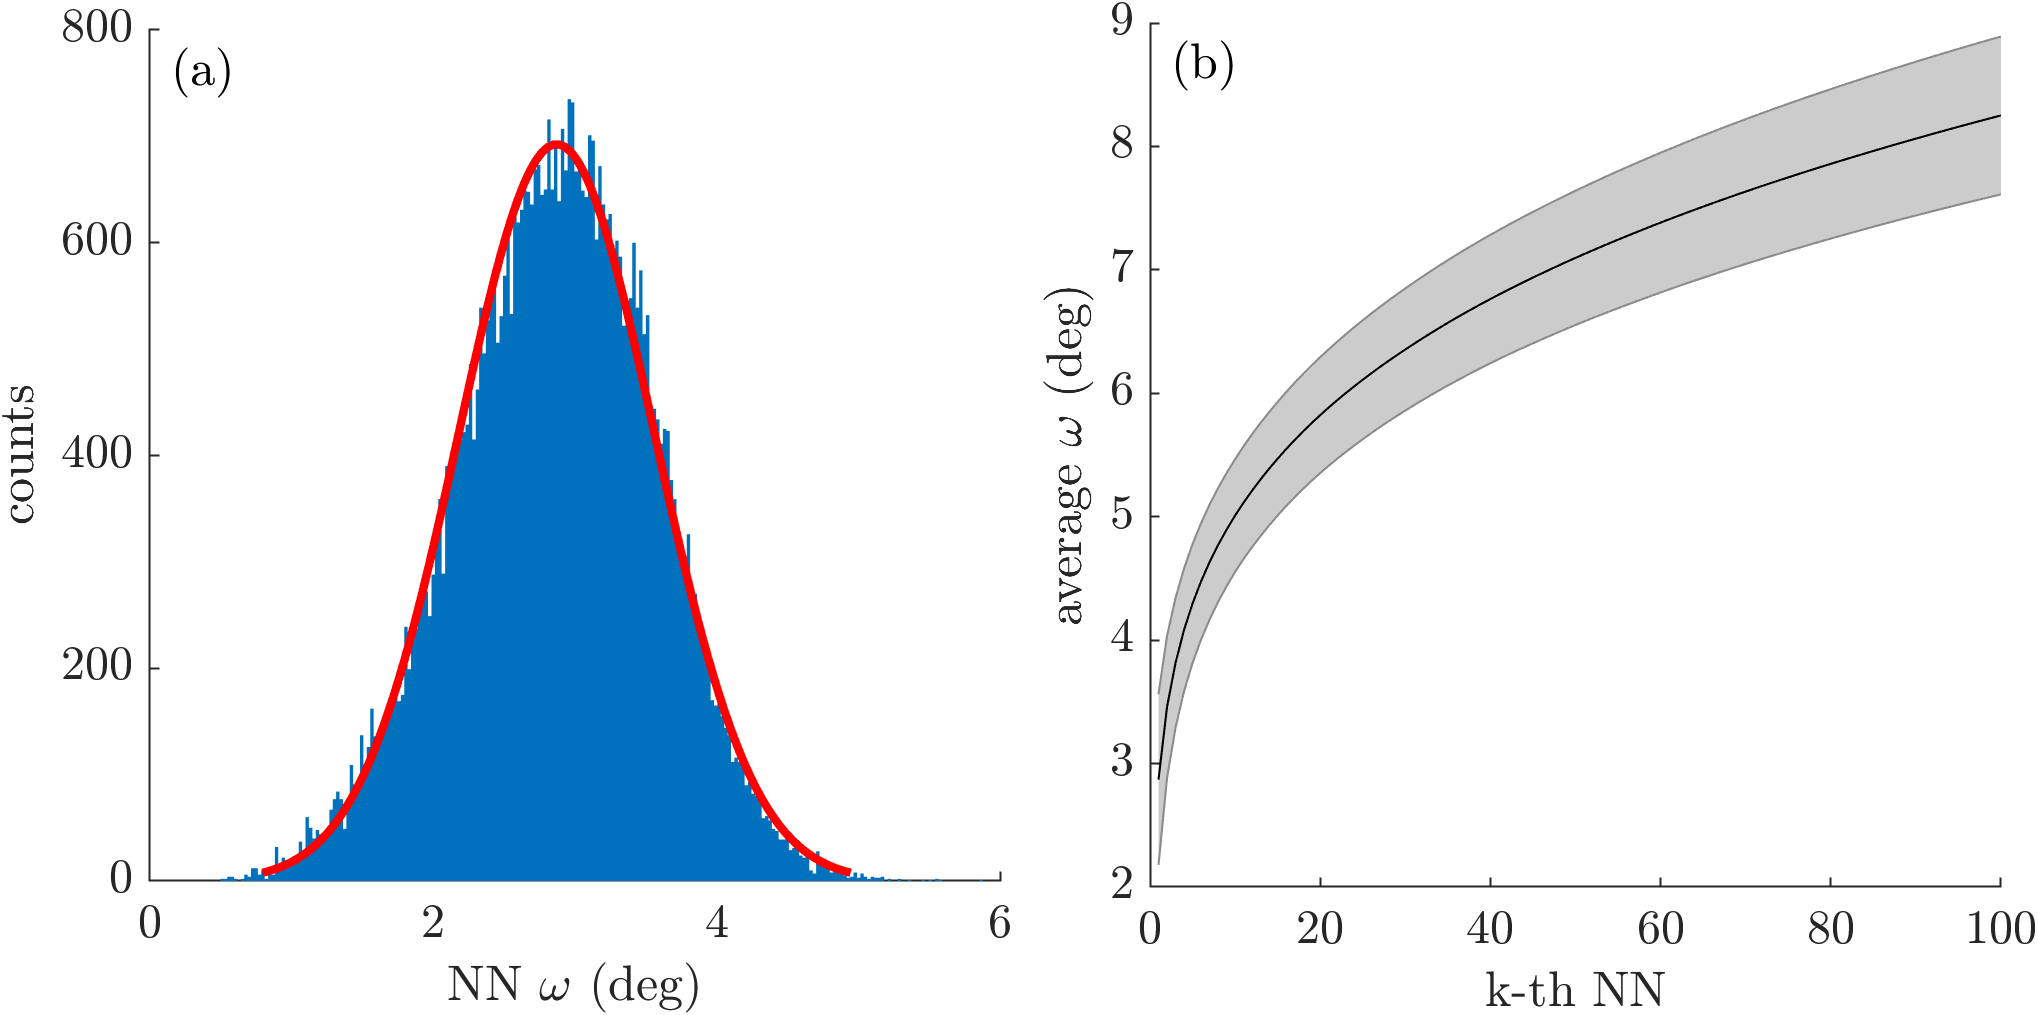
\includegraphics[scale=1]{nnhist-knn-50000.png}
% 		\caption{(a) Histogram of \gls{nn} \gls{gbo} distances ($\omega$) in a \gls{vfzgbo} set of \num{50000} points. The average \gls{nn} distance was \SI{\nnomega}{\degree}. (b) The average k-th nearest neighbor distances demonstrate that \glspl{nn} up to the $\sim$\num{10}-th \gls{nn} fall within a tolerance of $\sim$\SI{5}{\degree}. Standard deviation uncertainty bars using approximately 10 trial runs are also shown. }
% 		\label{fig:nnhist-knn-50000}
% 	\end{figure*}


\section{Semivariograms for Estimating Global and Local Correlation Lengths} \label{sec:supp:semivariogram}

    \subsection{Semivariogram Method}

    First, we provide some background to put correlation lengths in context. The construction of \gls{gpr} models involves the combination of a prior distribution over the model space, with some set of observations and their quantified uncertainty. The result is a posterior distribution that provides the probability (density) of any particular model in light of the observed data and priors. In \gls{gpr}, as the name suggests, the priors are assumed to be Gaussian and therefore of the form
    \begin{equation}
        f\!\left(\mathbf{m}\right) \propto \exp{\left(-\frac{1}{2} {\left(\mathbf{m}-\mathbf{m}_0\right)}^{\mathsf{T}} \mathbf{C}_{\mathbf{m}_0}^{-1} {\left(\mathbf{m}-\mathbf{m}_0\right)}\right)}
    \end{equation}
    where $f\!\left(\mathbf{m}\right)$ is the probability density of an arbitrary model, $\mathbf{m} = \mathbf{m}\!\left(x\right)$, and $\mathbf{m}_0 = \mathbf{m}_0\!\left(x\right)$ is the prior model (i.e. a guess as to what the true model ought to look like). The quantity $\mathbf{C}_{\mathbf{m}_0} = \mathbf{C}_{\mathbf{m}_0}\!\left(x_i,x_j\right)$ is the "kernel" or covariance function of the prior and it describes the prior (assumed) covariance between the values $\mathbf{m}\!\left(x_i\right)$ and $\mathbf{m}\!\left(x_j\right)$.
    
    It is possible to use a wide variety of kernel types, depending on the prior information one may have about the physical phenomenon one is attempting to model, e.g. continuity, differentiability, anisotropy, stationarity, and length-scales of correlation. One of the most common kernels employed is the Gaussian (sometimes called the squared exponential) kernel:
    \begin{equation} \label{eq:squared-exponential}                                                                                                                  σ  and σ , and \gls{vfz} coordinates, respectively.
	\left.\text{k[}x_i,x_j\text{$|\theta $]=}\sigma _f{}^2\text{Exp[-}\frac{1}{2}\frac{\left(x_i-x_j\right)\mathsf{T}\left(x_i-x_j\right)}{\sigma _l{}^2}\right]      f       l
\end{equation}
where $\sigma _f$, $\sigma _l$, $\theta$, and $x$ represent signal standard deviation, length scale (i.e. correlation length), unconstrained parameterization of 
    
    % estimate $\sigma$ and $l$ from the data.
    The values of $\sigma$ and $l$ are typically estimated from the data. One approach, employed by the \texttt{fitrgp()} routine in MATLAB involves numerical optimization via gradient descent which maximizes the likelihood as a function of these parameters \cite{ExactGPRMethod}.
    
    % or estimate using empirical semivariograms with a stationary Gaussian kernel.
    An alternative approach, adapted from geostatistical applications, involves calculation of the empirical semivariogram [REF], in which one bins the space of pairwise distances between all GBs and then calculates half the average pairwise variance of the corresponding property values in each bin:
    \begin{equation}
        \label{eq:semivariogram}
        \kappa\!\left(d_k\right) = \frac{1}{2N_k} \sum_{\substack{d_\Omega\left(x_i,x_j\right) \in \\ \left[d_k^-,d_k^+\right]}} {\left| E\!\left(x_i\right) - E\!\left(x_j\right)\right|}^2
    \end{equation}
    where $x_i$ and $x_j$ are the crystallographic coordinates of GBs $i$ and $j$, $d_\Omega\left(x_i,x_j\right)$ is the distance between them, and $E\!\left(x_i\right)$ and $E\!\left(x_i\right)$ are their respective energies. $d_k$ is the location (distance) of the $k$-th bin center having left- and right-hand limits $d_k^-$ and $d_k^+$, and $N_k$ is the number of measurement pairs whose distance falls in the $k$-th bin. Due to limited sampling of large distances and the fact that the most informative part of the semivariogram is the region near $d_k = 0$, it is customary to limit the semivariogram to half of the maximum distance [REF]. The empirical semivariogram is then fit with an analytical model to obtain the parameters of the kernel (covariance) function taking advantage of the relationship
    \begin{equation}
        \label{eq:analyticalsemivariogrammodel}
        \kappa\!\left(d\right) = \sigma_f^2 - \mathbf{C}_{\mathbf{m}_0}\!\left(d\right)
    \end{equation}
    where we have made explicit the stationarity of the Gaussian kernel (i.e. that it depends only the distance between two points, not on their respective locations).
    
    % choice of correlation strength
    Having obtained a value for the length scale kernel parameter $l$, one can define a correlation length for the data. If the distance between two points is equal to $l$ the kernel function indicates that their correlation will be equal to $\rho = \exp{\left(-1/2\right)} \approx 0.61$. However, one might reasonably want to know the length scale over which GB properties are correlated by a different amount. In general for a specified correlation strength, $\rho$, the corresponding correlation length is given by
    \begin{equation}
        \label{eq:generalizedcorrelationlength}
        l'\!\left(\rho\right) = l \sqrt{-2 \ln{\rho}}
    \end{equation}
    We will refer to the parameter $l$ as \emph{the} correlation length, but one can use \cref{eq:generalizedcorrelationlength} to determine the length scale corresponding to any specified correlation strength. %1-2 paragraphs

    \subsection{Global Correlation Lengths} \label{sec:supp:semivariogram:global}
	One of the most fundamental observations comes from the shape of the empirical semivariograms. As mentioned in \cref{sec:methods:correlation}, there are a wide variety of kernels that could be candidates for modeling correlations in different systems. Different kernels are used to capture different types of correlations, and each has a characteristic signature that can be observed in the semivariogram. For example, when a system exhibits exponential-type correlations, the semivariogram manifests this in the form of an exponential convergence towards an asymptotic constant value at long-distances. Linear and power-type correlations manifest an absence of a long-distance plateau. In the present system, there is a clear change in concavity in the semivariogram, this is a signature of correlations that are Gaussian in nature. Thus, we find that GB energy correlations in these systems are Gaussian, and should therefore be modeled using Gaussian kernels.
	\begin{figure*}
	    \centering
	    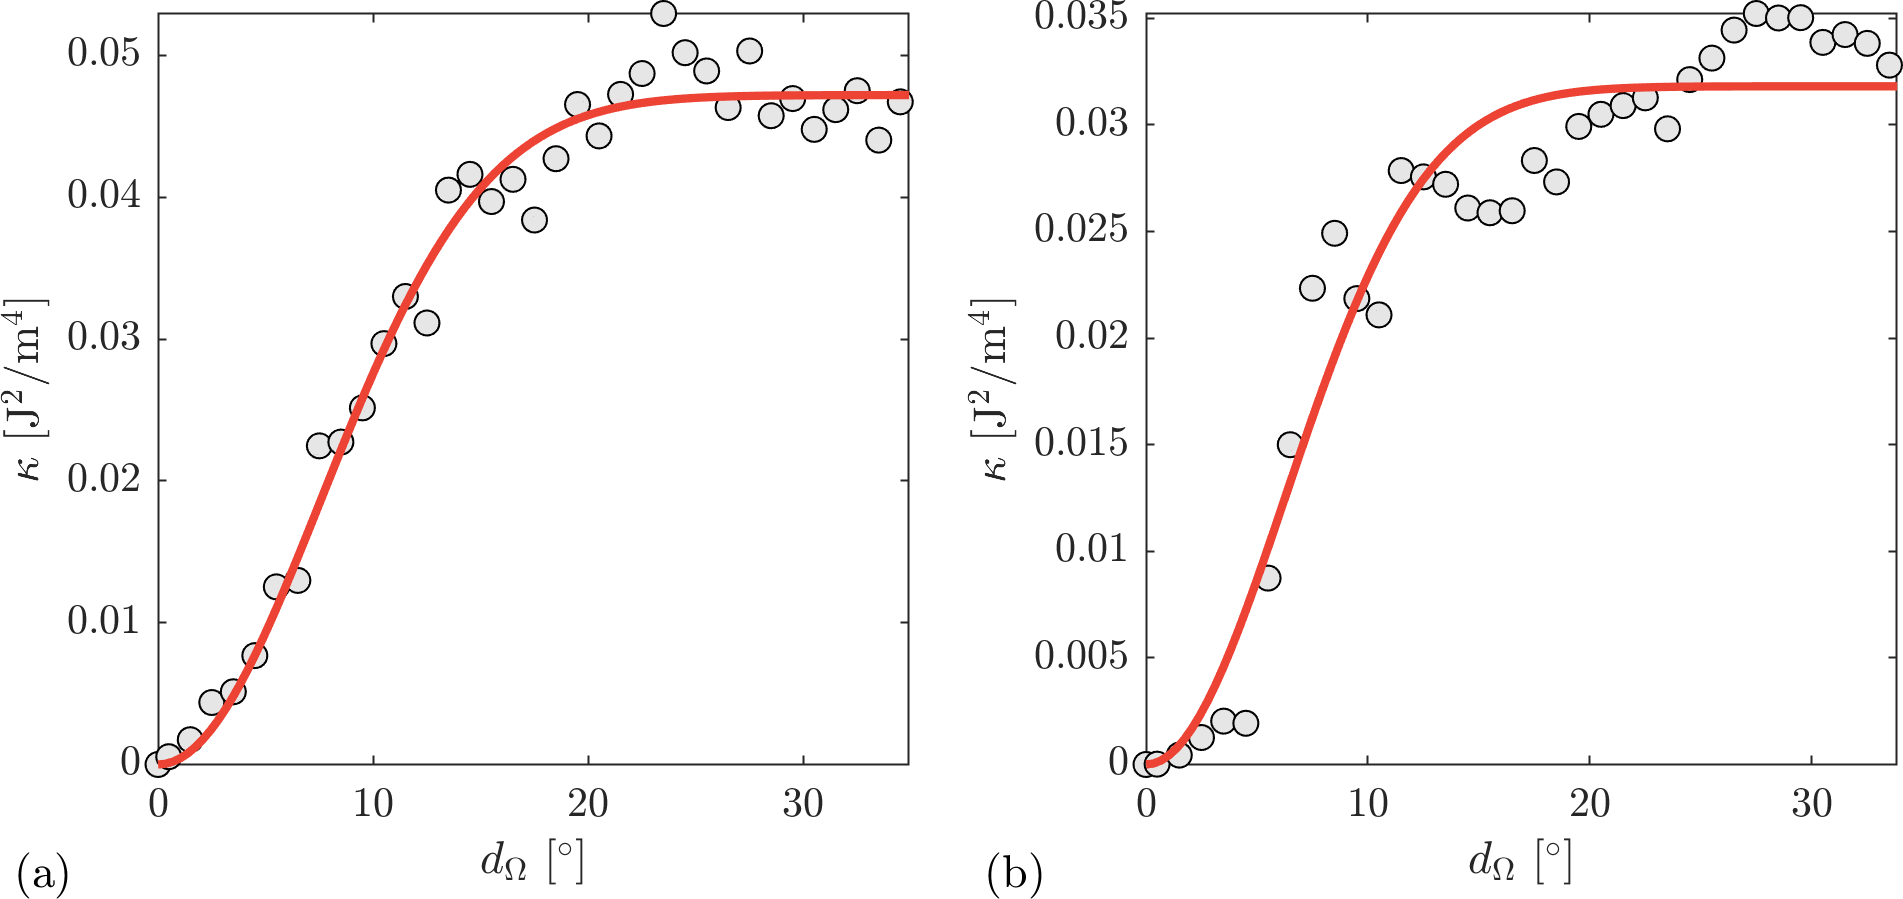
\includegraphics[scale=0.75]{figures/GlobalCorrelationLengthVariograms.png}
	    \caption{Empirical semivariograms (markers) for the (a) Ni and (b) Fe datasets. Solid lines show the fits of the analytical semivariogram models (\cref{eq:analyticalsemivariogrammodel}).}
	    \label{fig:globalvariogramfits}
	\end{figure*}
	
	\subsection{Local Correlation Lengths} \label{sec:supp:semivariogram:local}

    \begin{figure*}
        \centering
        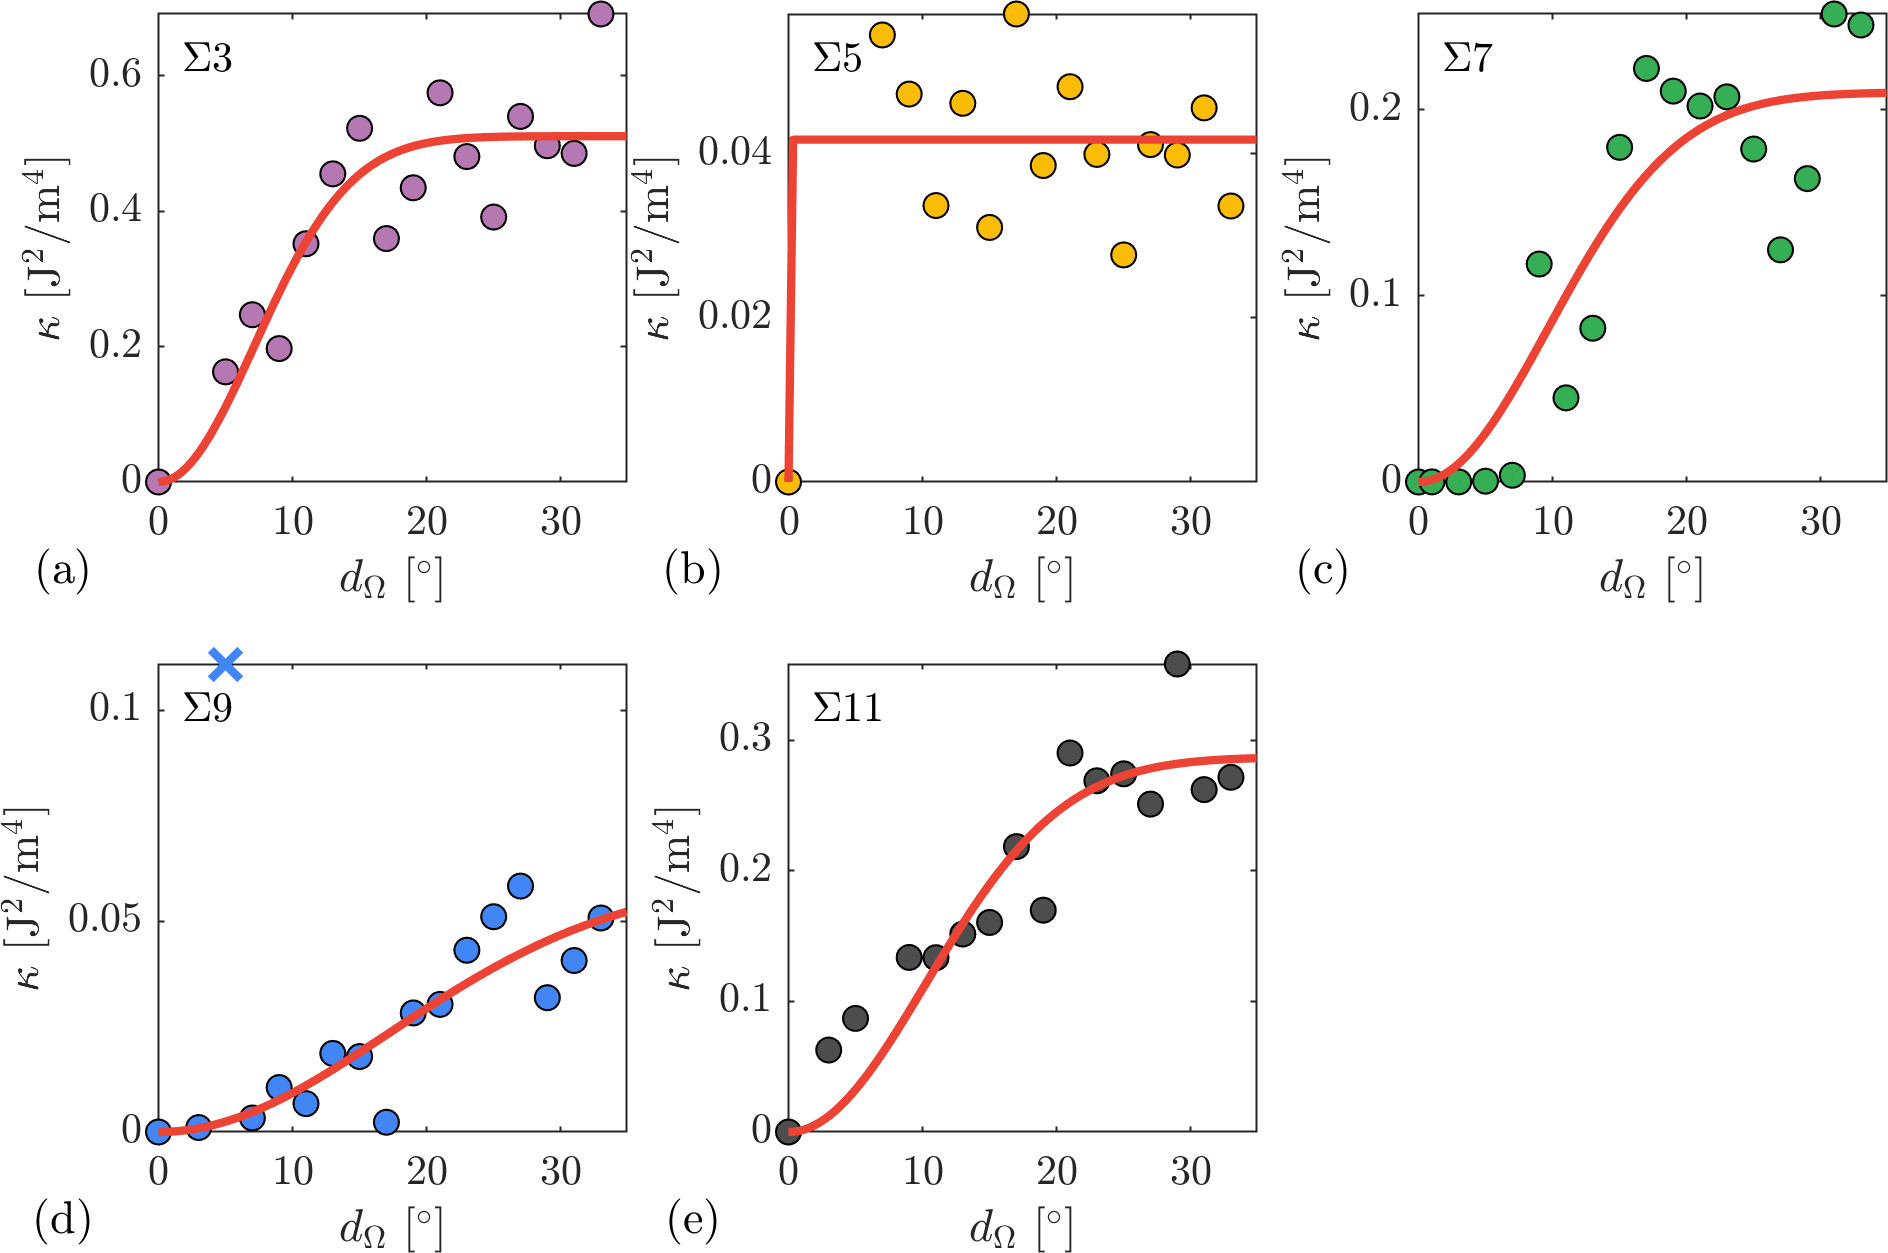
\includegraphics[scale=1]{figures/LocalCorrelationLengthVariogramsOlmsted.png}
        \caption{Local empirical semivariograms (markers), respectively centered at various low-$\Sigma$ GBs for the Ni dataset. Solid lines show the fits of the analytical semivariogram models. In (d) the one point marked with an $\times$ was considered an outlier and was excluded from the fit.}
        \label{fig:localvariogramsolmsted}
    \end{figure*}
    \begin{figure*}
        \centering
        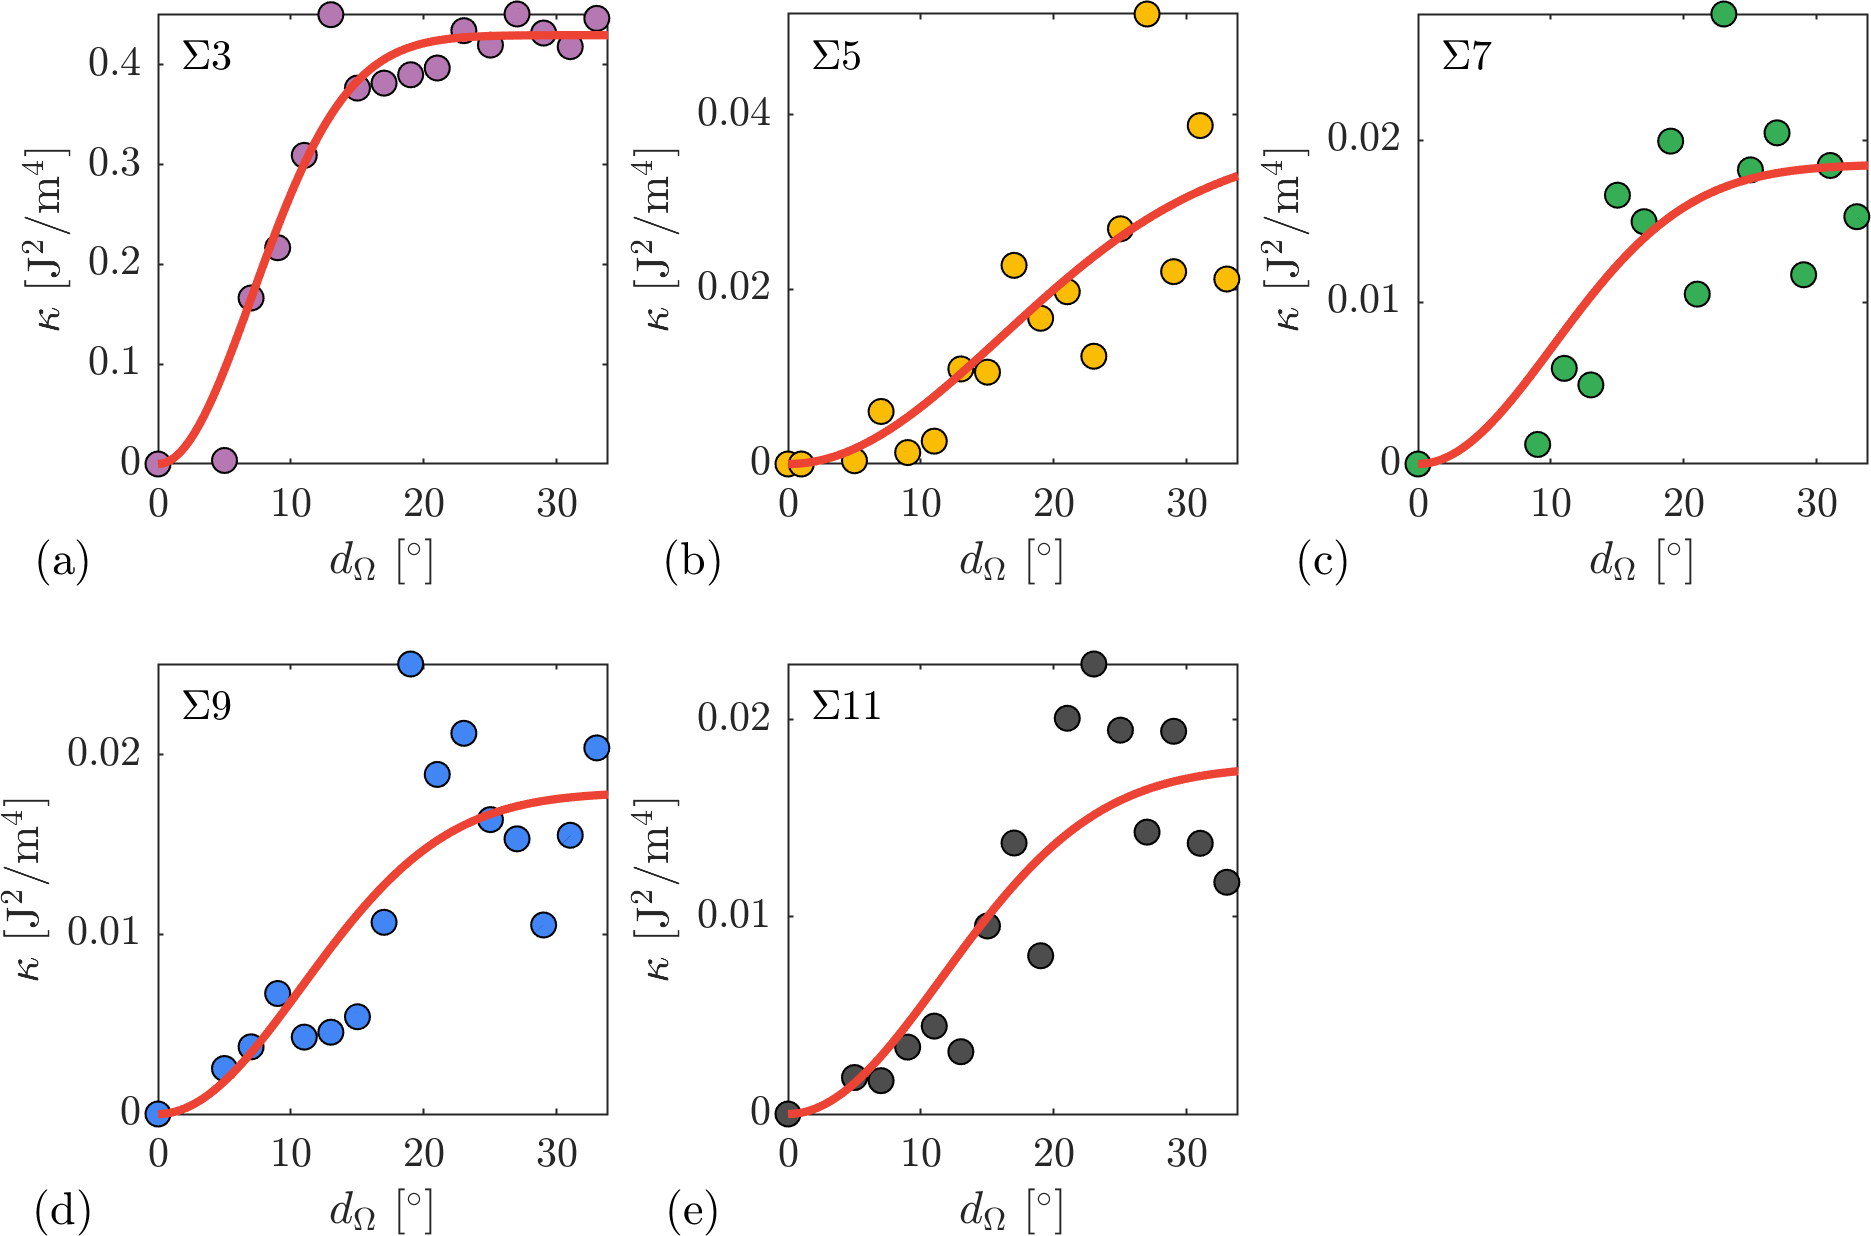
\includegraphics[scale=1]{figures/LocalCorrelationLengthVariogramsKim.png}
        \caption{Local empirical semivariograms (markers), respectively centered at various low-$\Sigma$ GBs for the Fe dataset. Keys for which \glspl{gb} each of these correspond to in the original papers are given for Fe and Ni in \cref{tab:sigma-key-olmsted,tab:sigma-key-kim}, respectively. Solid lines show the fits of the analytical semivariogram models.}
        \label{fig:localvariogramskim}
    \end{figure*}
    The local empirical semivariograms are noisier than the global empirical semivariograms, likely due to considering fewer GB pairs. Nevertheless, reasonable fits were obtained for most of the GBs with the exception of the $\Sigma 5$ GB in the Ni dataset. In many of the local semivariograms we again see the signature change in concavity suggesting that the local correlations in the vicinity of these GBs are also Gaussian in nature. However, there are some exceptions where the nature of the correlations is more ambiguous. We anticipate that this ambiguity could be resolved with datasets that are either larger (compared to the Ni dataset) or having less noise (compared to the Fe dataset) than those considered here. However, the local empirical semivariograms seem to be generally consistent with Gaussian-type correlations.
    
    The traditional Gaussian kernel exhibits the property of stationarity, meaning that the covariance depends only on the distance between two points, not on their respective locations (i.e. $\mathbf{C}_{\mathbf{m}_0}\!\left(x_i,x_j\right) = \mathbf{C}_{\mathbf{m}_0}\!\left(d\left(x_i,x_j\right)\right)$). The use of a stationary kernel implies a prior assumption that there is a single global correlation length that applies everywhere. The fact that we observe significant variation in correlation length across the \gls{gb} character space suggests that it would be better to employ non-stationary kernels (this is why, when referring to the global correlation length results presented earlier, we were careful to say that the global correlation lengths hold "on average" across the space). In particular, due to the fact that the local semivariograms do seem to be generally consistent with Gaussian-type correlations, we suggest that the non-stationary version of the Gaussian kernel [REF] may be a reasonable choice. One additional potential benefit of employing non-stationary kernels might be improved resolution of cusps in the \gls{gb} energy landscape.

\section{Fe Input Data Quality}
	\label{sec:supp:kim-interp:quality}
	Of the $\sim$\num{60000} \glspl{gb}\footnote{The "no-boundary" \glspl{gb} (i.e. \glspl{gb} with close to \SI{0}{\joule\per\square\meter} \gls{gbe}) were removed before testing for degeneracy.} in \cite{kimPhasefieldModeling3D2014}, $\sim$\num{10000} \glspl{gb} were repeats that were identified by converting to \glspl{vfzgbo} and applying \vfzorepo{} function \texttt{avg\_repeats.m}. In \cite{kimPhasefieldModeling3D2014}, mechanically selected \glspl{gb} were those which involved sampling in equally spaced increments\footnote{In some cases, this was equally spaced increments of the argument of a trigonometric function.} for each \gls{5dof} parameter, and a few thousand intentionally selected \glspl{gb} (i.e. special \glspl{gb}) were also considered. Of mechanically and intentionally selected \glspl{gb}, \numlist{9170;112} are repeats, respectively, with a total of \num{2496} degenerate sets\footnote{A degenerate "set" is distinct from a \gls{vfzgbo} "set", the latter of which is often used in the main text.} (see \cref{fig:kim-interp-degeneracy-sets} for a degeneracy histogram). Thus, on average there is a degeneracy of approximately four per set of degenerate \glspl{gb}.
	
	By comparing \gls{gbe} values of (unintentionally\footnote{To our knowledge, the presence of repeat \glspl{gb} were not mentioned in \cite{kimPhasefieldModeling3D2014} or \cite{kimIdentificationSchemeGrain2011}}) repeated \glspl{gb} in the Fe simulation dataset \cite{kimPhasefieldModeling3D2014}, we can estimate the intrinsic error of the \inpt{} data. For example, minimum and maximum deviations from the average value of a degenerate set are \SIlist{-0.2625;0.2625}{\joule\per\square\meter}, respectively, indicating that a repeated Fe \gls{gb} simulation from \cite{kimPhasefieldModeling3D2014} can vary by as much as \SI{0.525}{\joule\per\square\meter}, though rare. Additionally, \Gls{rmse} and \gls{mae} values can be obtained within each degenerate set by comparing against the set mean. Overall \gls{rmse} and \gls{mae} are then obtained by averaging and weighting by the number of \glspl{gb} in each degenerate set. Following this procedure, we obtain an average set-wise \gls{rmse} and \gls{mae} of \SIlist{0.06529;0.06190}{\joule\per\square\meter}, respectively, which is an approximate measure of the intrinsic error of the data. \cref{fig:kim-interp-degeneracy-results} shows histograms and parity plots of the intrinsic error. The overestimation of intrinsic error mentioned in the main text (\cref{sec:results:lit:error}) could stem from bias as to what type of \glspl{gb} exhibit repeats based on the sampling scheme used in \cite{kimPhasefieldModeling3D2014} and/or that many of the degenerate sets contain a low number of repeats (\cref{fig:kim-interp-degeneracy-sets}).
	
	Next, we see that by binning \glspl{gb} into degenerate sets, most degenerate sets have a degeneracy of fewer than 5 \cref{fig:kim-interp-degeneracy-sets}. We split the repeated data into sets with a degeneracy of fewer than 5 and greater than or equal to 5 and plot the errors (relative to the respective set mean) in both histogram form (\cref{fig:kim-interp-degeneracy-results}a and \cref{fig:kim-interp-degeneracy-results}c, respectively) and as hexagonally-binned parity plots (\cref{fig:kim-interp-degeneracy-results}b and \cref{fig:kim-interp-degeneracy-results}d, respectively). While heavily repeated \glspl{gb} tend to give similar results, occasionally repeated \glspl{gb} often have larger \gls{gbe} variability. This could have physical meaning: Certain types of (e.g. high-symmetry) \glspl{gb} tend to have less variation (i.e. fewer and/or more tightly distributed metastable states). However, it could also be an artifact of the simulation setup that produced this data (e.g. deterministic simulation output for certain types of \glspl{gb}).
	
	\begin{figure}
		\centering
		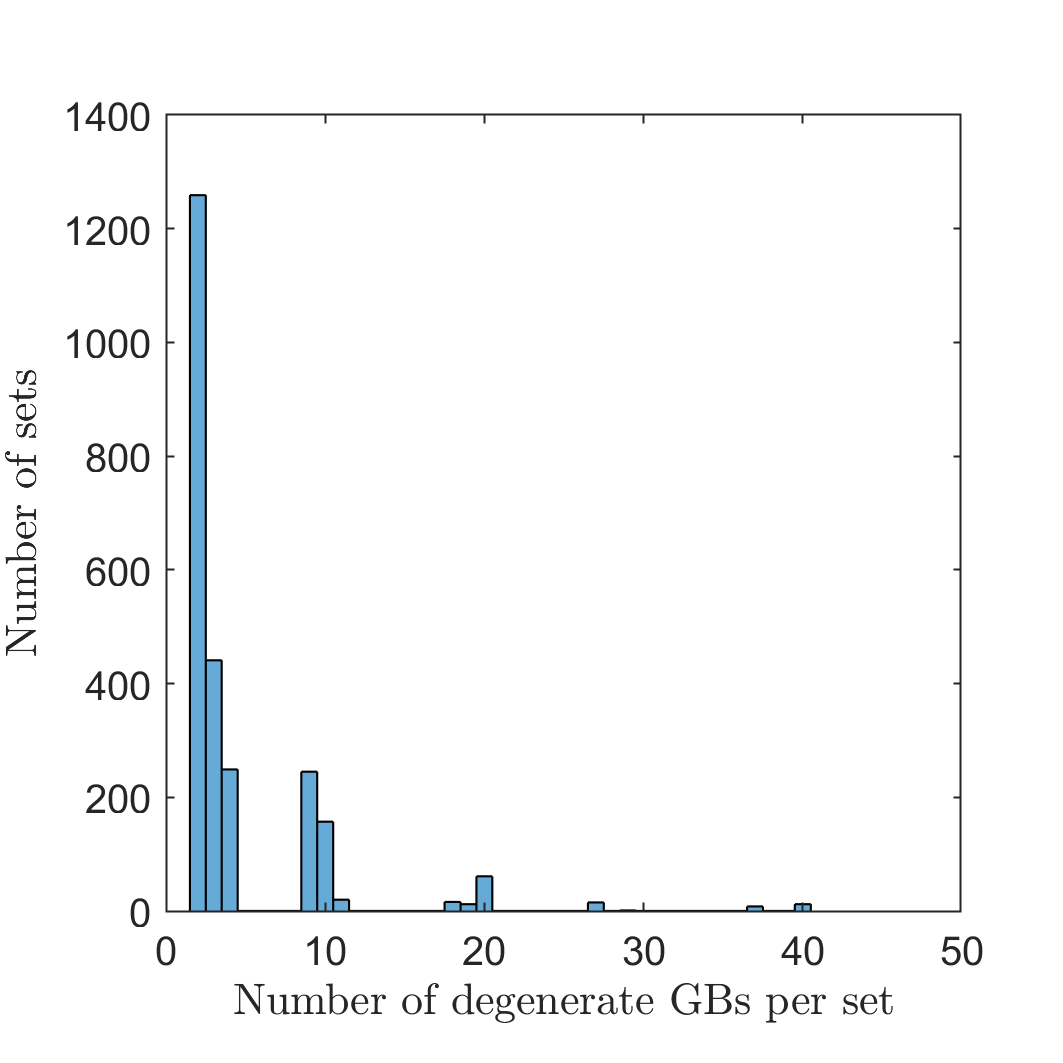
\includegraphics[scale=1]{kim-interp-degeneracy-sets.png}
		\caption{Histogram of number of sets vs. number of degenerate \glspl{gb} per set for the Fe simulation dataset \cite{kimPhasefieldModeling3D2014}. Most sets have a degeneracy of fewer than 5.}
		\label{fig:kim-interp-degeneracy-sets}
	\end{figure}
	
	\begin{figure}
		\centering
		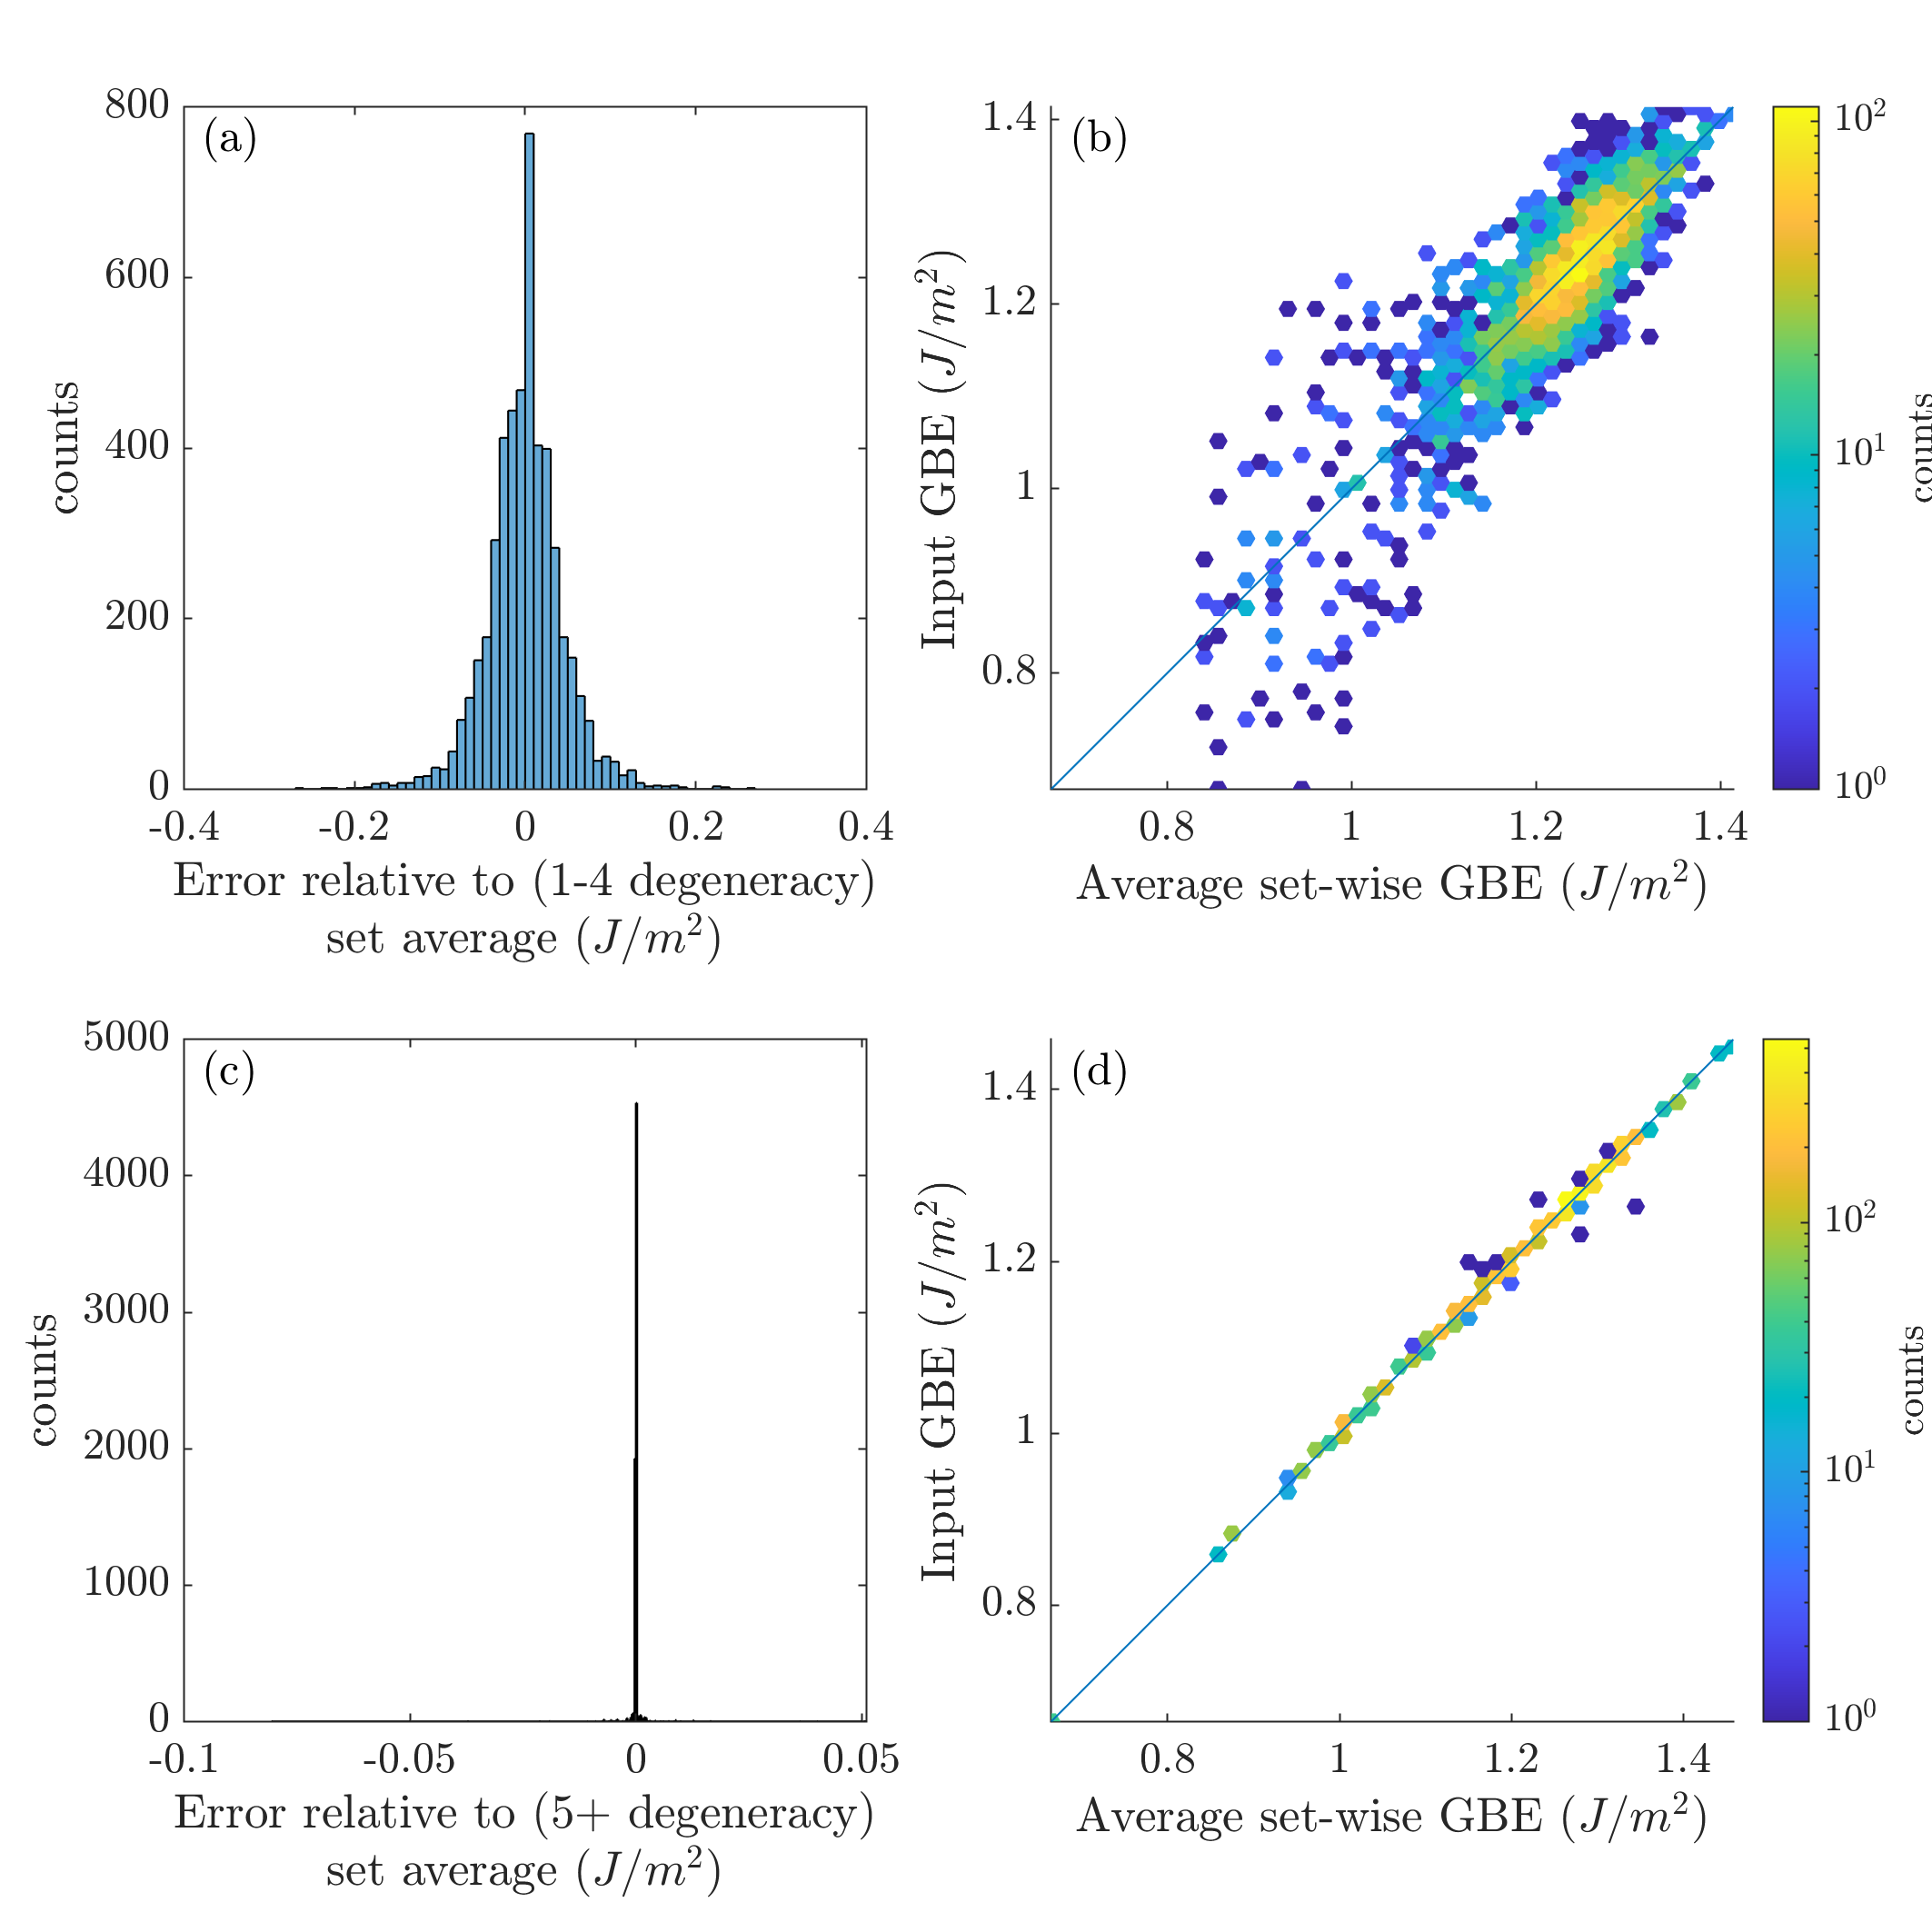
\includegraphics[scale=1]{kim-interp-degeneracy-results.png}
		\caption{Degenerate \glspl{gb} sets are split into those with a degeneracy of fewer than 5 and greater than or equal to 5 and plotted as ( (a) and (c), respectively) error histograms and ( (b) and (d), respectively) hexagonally-binned parity plots. Large degenerate sets tend to have very low error, whereas small degenerate sets tend to have higher error. In other words, \glspl{gb} that are more likely to be repeated many times based on the sampling scheme in \cite{kimPhasefieldModeling3D2014} tend to give similar results, whereas \glspl{gb} that are less likely to be repeated often have larger variability in the simulation output. We do not know if this has physical meaning or is an artifact of the simulation setup.}
		\label{fig:kim-interp-degeneracy-results}
	\end{figure}

\section{Gridded Sampling for Numerical Differentation} \label{sec:supp:grid}
An isotropically sized \gls{fz} may be easier to uniformly discretize than a high aspect-ratio space (i.e. a fixed discretization length can be used across all dimensions). What this doesn't describe, however, is curvature. In order to create a gridded array, which is important for numerical differentiation, a hypercube with each primary axis oriented with Euclidean dimensions is to be preferred. As curvature or misalignment is introduced as may be expected with a \gls{vfz} point cloud, \glspl{gb} outside of the \gls{vfz} will necessarily be sampled; this phenomena will be exaggerated in high dimensions\footnote{For perspective, a discretization into 9 segments (10 points) along each dimension will have a spacing of $\sim$\SI{7}{\degree} and require \num{1e5} grid points. In order to achieve a more reasonable grid spacing of $\sim$\SI{2}{\degree}, a minimum of $\sim$\num{24} discretizations (25 points) along each dimension is necessary and will produce $\sim$\num{1e7} grid points. }. Fortunately, most of the information is contained in the first five dimensions after \gls{svd} transformation (\cref{sec:results:dimensions}). Thus, the latter three dimensions can likely be ignored without substantially affecting e.g. an interpolation or numerical differentiation scheme.

\section{\glsxtrshort{gb}s Used for Path Visualization} \label{sec:supp:sigma-key}

See \cref{tab:sigma-key-olmsted} and \cref{tab:sigma-key-kim} for the \citet{olmstedSurveyComputedGrain2009} and \citet{kimPhasefieldModeling3D2014} datasets, respectively.

\begin{table}[!htb]
    \centering
    \caption{Minimum $\Sigma$ (Sigma) \glspl{gb} and corresponding IDs used for path visualization within the original \citet{olmstedSurveyComputedGrain2009} dataset. }
    \label{tab:sigma-key-olmsted}
    \csvautobooktabular{tables/sigma-key-olmsted.csv}
\end{table}

\begin{table}[!htb]
    \centering
    \caption{Minimum $\Sigma$ (Sigma) \glspl{gb} and corresponding IDs used for path visualization within the original \citet{kimPhasefieldModeling3D2014} dataset. }
    \label{tab:sigma-key-kim}
    \csvautobooktabular{tables/sigma-key-kim.csv}
\end{table}

\printglossary

\clearpage
\bibliographystyle{elsarticle-num-names}
\bibliography{5dof-gb-energy.bib}

\end{document}